\section{Successful interactions and patches}
\label{sec:patches}

\subsection{The successful-interaction skeleton}

A nonempty-target interaction \((i,t,\alpha,S)\), with
\(\alpha\in\{\delta,\beta\}\), is \emph{successful} when its source is
active immediately before it occurs:
\[
  i\in A_{t-}.
\]
Its skeleton is the triple \((i,t,S)\); in particular, it does not
reveal whether the interaction is a split or a birth.  The initial
interaction is declared successful and has skeleton
\((\infty,0,A)\).

For \(T<\infty\), let \(\cI_T\) be the initial skeleton together with
all ordinary successful-interaction skeletons through time \(T\), and
put
\begin{equation}
  \cG_T=\sigma\bigl((A_0,\sigma_0),\cI_T\bigr).
  \label{eq:skeleton-sigma-field}
\end{equation}
Deaths have empty target and are not included in \(\cI_T\).

\subsection{Patches}

A successful interaction \((i,t,S)\) touches \(i\) as an outgoing
touch and each \(j\in S\) as an incoming touch.  At each site, order
all successful touches in time.  A patch is the site-time interval
between two successive touches, together with four labels:
\[
  P
  =
  \{i(P)\}\times[s(P),e(P))
  \times\{\mathsf X(P)\mathsf Y(P)\}
  \times\{S(P)\}.
\]
The initial label is \(\sI\) when \(i(P)\in S(P)\) and \(\sO\)
otherwise.  The terminal label is \(\sI\) or \(\sO\) according to the
next touch, and is \(\sE\) when no later touch has yet been revealed.
At a finite horizon \(T\), patches ending before \(T\) are
\emph{bulk patches}; those cut by \(T\) are \emph{end patches}.  Their
families are denoted by \(\cB_T\) and \(\cE_T\), and
\[
  \cP_T=\cB_T\cup\cE_T.
\]
Every end patch is based at a distinct site of the interaction cone
\(\Cone_T\).

\begin{figure}[htbp]
  \centering
  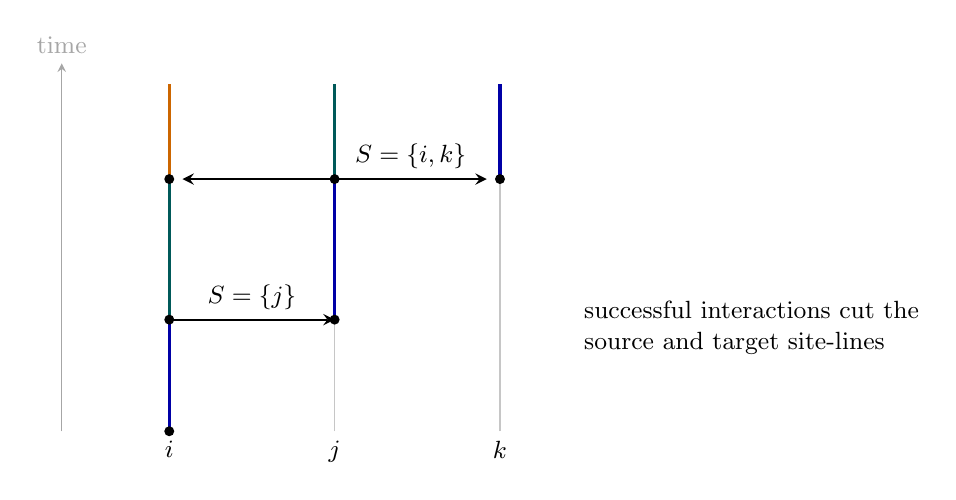
\begin{tikzpicture}[
  x=2.1cm,
  y=1.05cm,
  >=stealth,
  every node/.style={font=\small}
]
  \draw[->,gray!70] (-0.65,0) -- (-0.65,4.45) node[above] {time};

  \foreach \x/\lab in {0/\(i\),1/\(j\),2/\(k\)} {
    \draw[gray!45] (\x,0) -- (\x,4.2);
    \node[below] at (\x,0) {\lab};
  }

  \draw[very thick,blue!65!black] (0,0) -- (0,1.35);
  \draw[very thick,teal!70!black] (0,1.35) -- (0,3.05);
  \draw[very thick,orange!80!black] (0,3.05) -- (0,4.2);

  \draw[very thick,blue!65!black] (1,1.35) -- (1,3.05);
  \draw[very thick,teal!70!black] (1,3.05) -- (1,4.2);

  \draw[very thick,blue!65!black] (2,3.05) -- (2,4.2);

  \fill (0,0) circle (1.8pt);
  \fill (0,1.35) circle (1.8pt);
  \fill (1,1.35) circle (1.8pt);
  \fill (0,3.05) circle (1.8pt);
  \fill (1,3.05) circle (1.8pt);
  \fill (2,3.05) circle (1.8pt);

  \draw[->,thick] (0,1.35) -- (1,1.35)
    node[midway,above] {\(S=\{j\}\)};
  \draw[->,thick] (1,3.05) -- (0.08,3.05);
  \draw[->,thick] (1,3.05) -- (1.92,3.05)
    node[midway,above] {\(S=\{i,k\}\)};

  \node[left] at (-0.05,0.65) {\(\sI\sO\)};
  \node[left] at (-0.05,2.15) {\(\sO\sI\)};
  \node[right] at (1.05,2.15) {\(\sI\sO\)};
  \node[left] at (-0.05,3.65) {\(\sI\sE\)};
  \node[right] at (1.05,3.65) {\(\sO\sE\)};
  \node[right] at (2.05,3.65) {\(\sI\sE\)};

  \node[align=left,anchor=west] at (2.45,1.25)
    {successful interactions cut the\\source and target site-lines};
\end{tikzpicture}

  \caption{A successful interaction cuts the source and every target
  site-line.  The intervals between successive cuts are patches.  The
  first label records whether a patch begins at an incoming or
  outgoing touch; the second records its terminal touch or the finite
  horizon.}
  \label{fig:patch-schematic}
\end{figure}

\subsection{Reference patch laws and consistency}

Fix a labeled patch \(P\), abbreviate
\[
  i=i(P),\quad s=s(P),\quad e=e(P),\quad S=S(P),
\]
and consider all interactions outgoing from \(i\) in the open
interval \((s,e)\).  Under the reference law \(\pP_P\), these are the
original independent Poisson clocks restricted to \((s,e)\).  If
\(\mathsf X(P)=\sO\), the interaction at time \(s\) is also included;
its hidden kind has law
\begin{equation}
  \pP_P(\alpha=\delta)
  =
  \frac{\delta_i(S)}{\delta_i(S)+\beta_i(S)},
  \qquad
  \pP_P(\alpha=\beta)
  =
  \frac{\beta_i(S)}{\delta_i(S)+\beta_i(S)}.
  \label{eq:boundary-kind-law}
\end{equation}

These data generate a one-site active indicator \(X^P\).  An incoming
patch starts active.  An outgoing patch starts inactive after a split
and active after a birth.  Thereafter an empty-target death makes the
site inactive, a split makes it inactive, and a birth leaves it
active, provided the source was active.

The event \(\operatorname{Con}(P)\) requires two things:
\begin{enumerate}[(i)]
  \item every nonempty-target interaction strictly inside \(P\) has
  inactive source, so it does not create an unrecorded successful
  interaction;
  \item if \(\mathsf Y(P)=\sO\), then the source is active immediately
  before \(e(P)\).
\end{enumerate}
Incoming and end terminal labels impose no terminal activity
condition.  For every realized finite-horizon patch,
\(\pP_P(\operatorname{Con}(P))>0\) almost surely.  We write
\[
  \pP_P^{\mathrm{con}}(\,\cdot\,)
  =
  \pP_P(\,\cdot\mid\operatorname{Con}(P))
\]
for the consistent patch law.

\begin{theorem}[Finite-horizon patch factorization]
\label{thm:patch-factorization}
Fix \(T<\infty\).  Conditional on \(\cG_T\), the patch interaction
data are independent, and the conditional law in patch
\(P\in\cP_T\) is \(\pP_P^{\mathrm{con}}\).  Thus, for bounded
measurable \(f_P\),
\begin{equation}
  \E\left[
    \prod_{P\in\cP_T}f_P
    \,\middle|\,\cG_T
  \right]
  =
  \prod_{P\in\cP_T}
  \E_P^{\mathrm{con}}[f_P].
  \label{eq:patch-factorization}
\end{equation}
\end{theorem}

\begin{proof}
Fix a realization \(g\) of the finite skeleton.  It determines a
finite labeled family \(\cP_T(g)\) and finitely many boundary points.
Disintegrate the joint law of the ordered Poisson points at these
locations.  Independent increments on the disjoint source-time
intervals give the product reference law
\[
  \bigotimes_{P\in\cP_T(g)}\pP_P;
\]
at an outgoing boundary, the unrevealed mark has the proportional-rate
law \eqref{eq:boundary-kind-law}.

Relative to the fixed boundary points, the event that \(g\) is the
complete successful skeleton is precisely
\[
  \bigcap_{P\in\cP_T(g)}\operatorname{Con}(P).
  \tag{*}
\]
The forward implication follows from the definition.  For the reverse
implication, read the boundary interactions chronologically.  The
local indicators agree with the global active state between boundary
times; interior consistency rules out any missing successful
interaction; terminal consistency activates every recorded outgoing
boundary; and that boundary begins exactly the prescribed source and
target patches.  Induction reconstructs the global active process and
proves \((*)\).

Conditioning the product reference law on \((*)\) therefore gives
\[
  \frac{
    \prod_{P}
    \ind(\operatorname{Con}(P))\,\pP_P(\dd\Sigma_P)
  }{
    \prod_P\pP_P(\operatorname{Con}(P))
  }
  =
  \bigotimes_P\pP_P^{\mathrm{con}}(\dd\Sigma_P),
\]
which proves \eqref{eq:patch-factorization}.  Only finitely many
source-time strips are involved, so the infinite lattice introduces
no additional conditioning issue.
\end{proof}

\begin{remark}
The theorem is deliberately finite-horizon.  Infinite patches and
their limiting factors will be defined by endpoint limits; none of the
main results requires factorization conditional on an all-time
successful skeleton.
\end{remark}
